% !TEX root =  bopp.tex


\begin{figure*}[p]
	\centering
	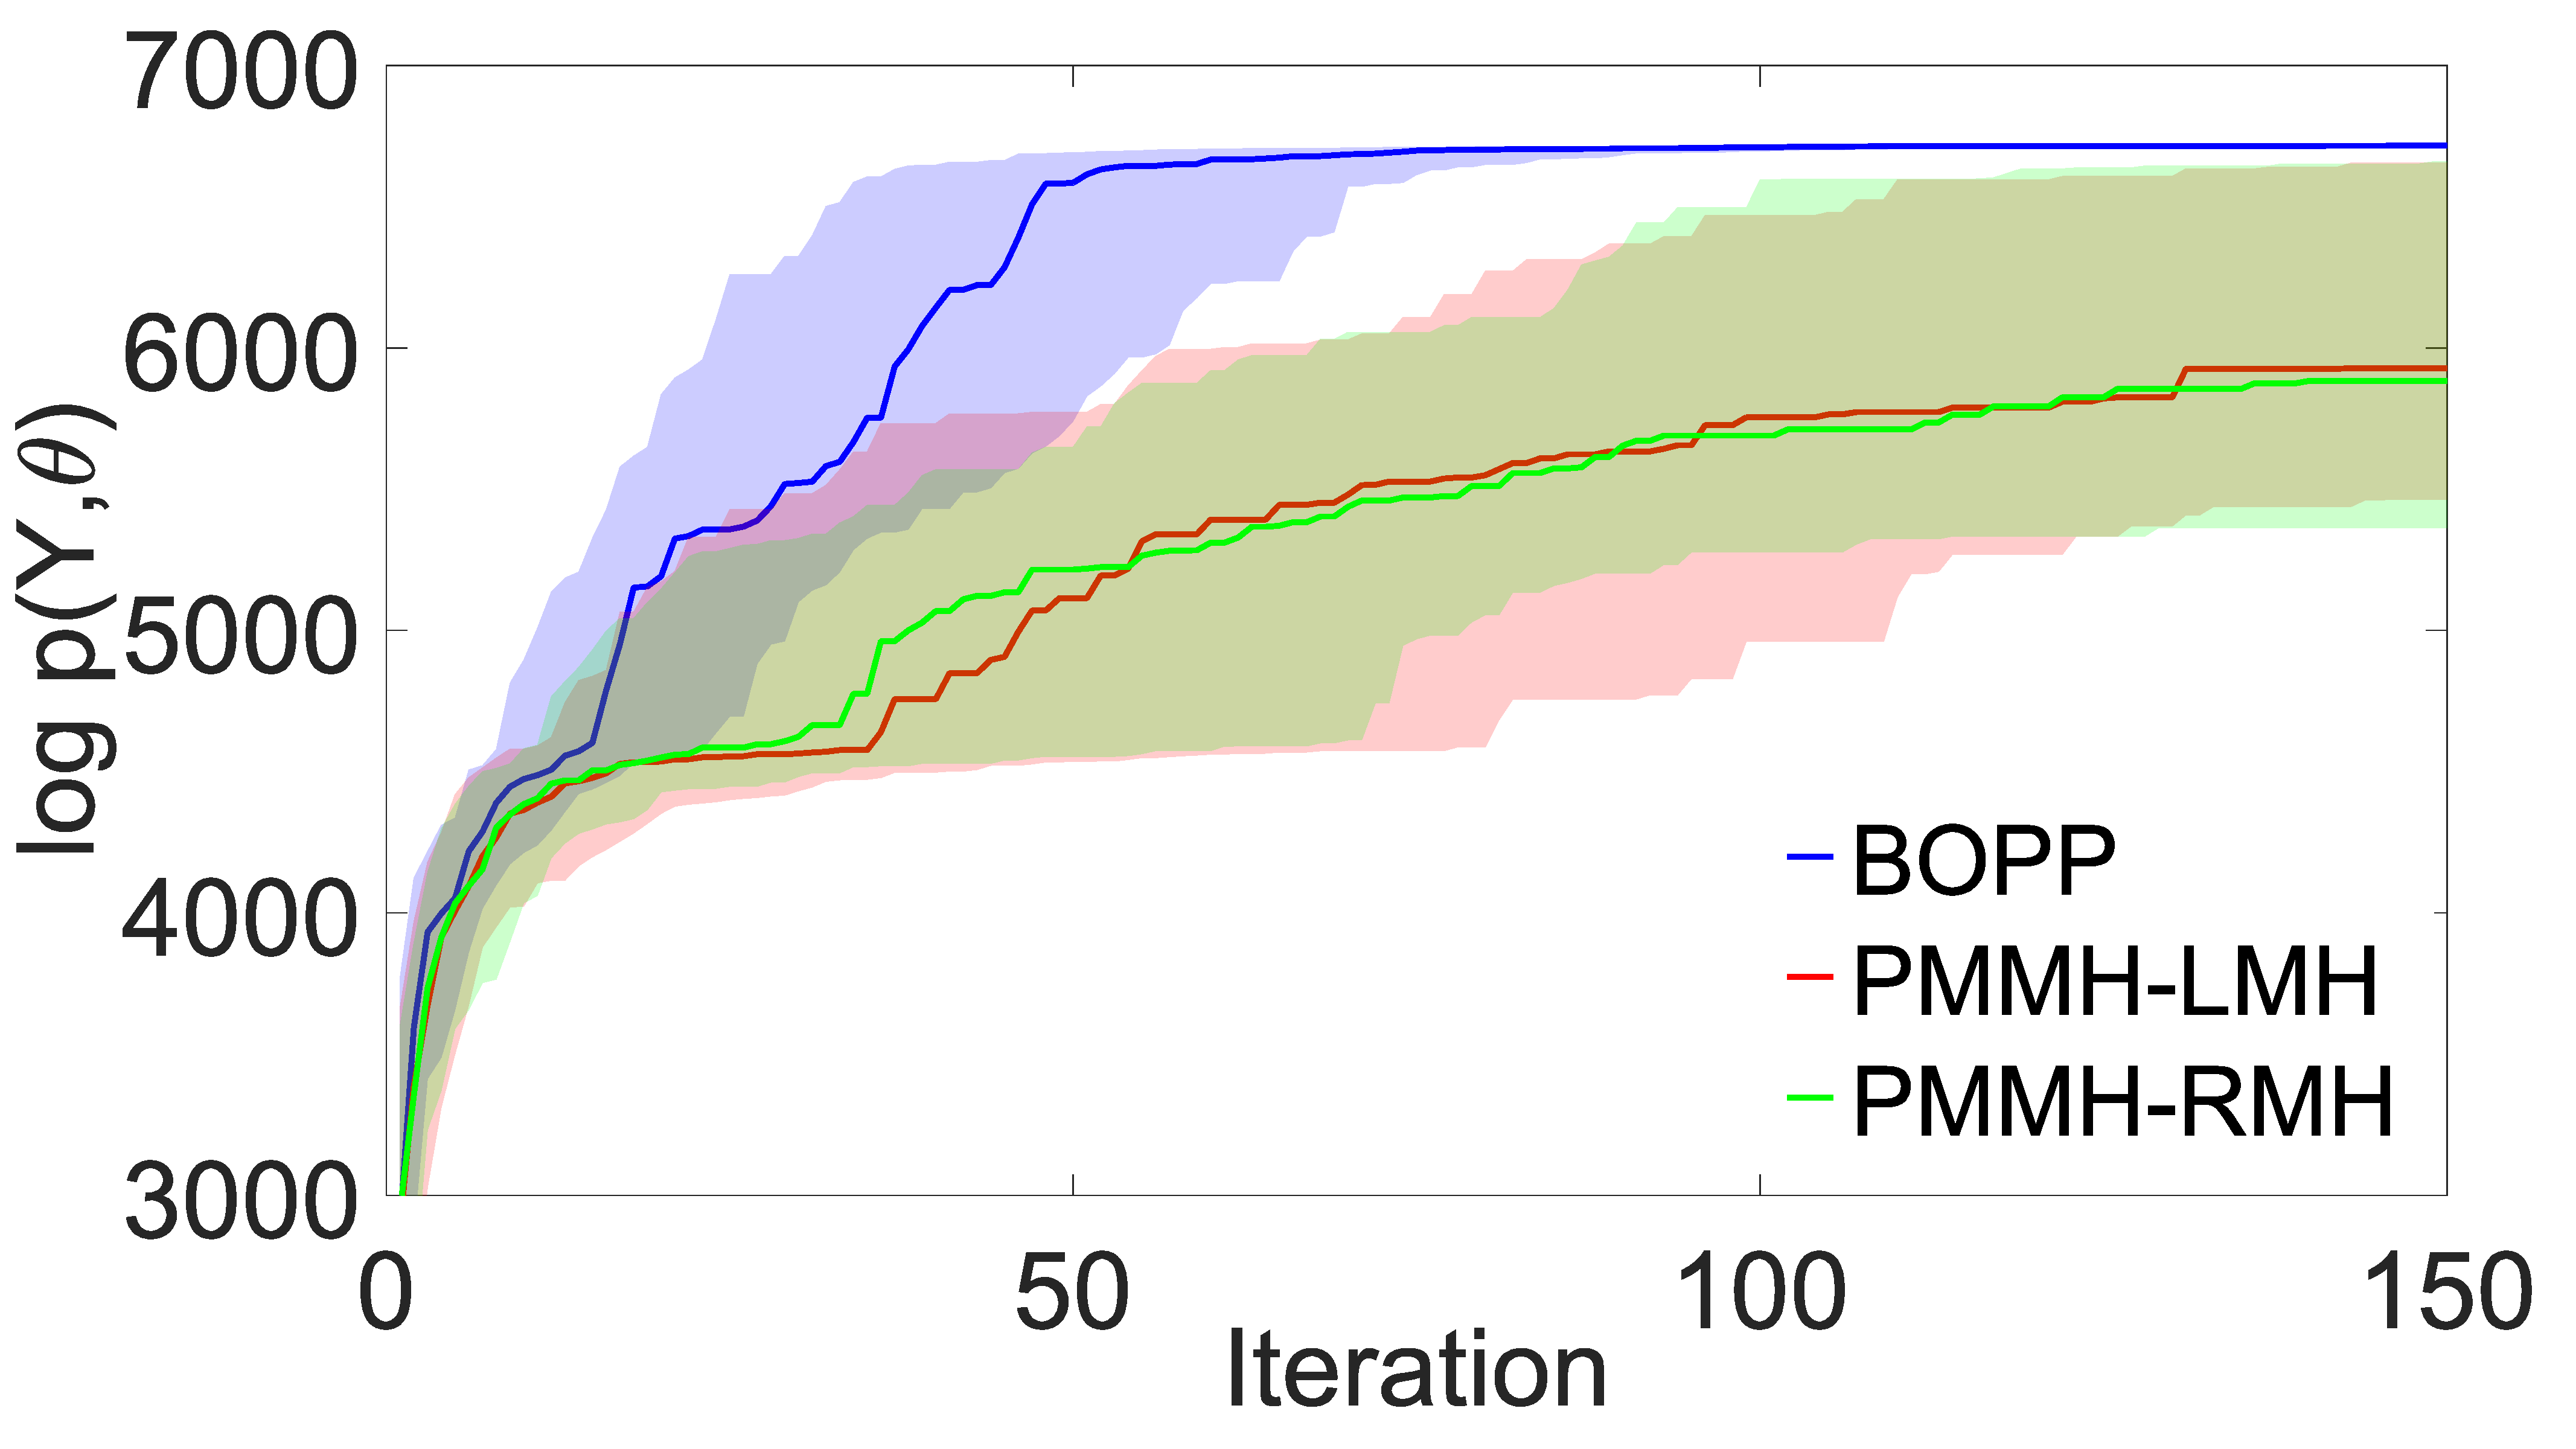
\includegraphics[width=2.72in]{chaos/chaos_ml.pdf}
	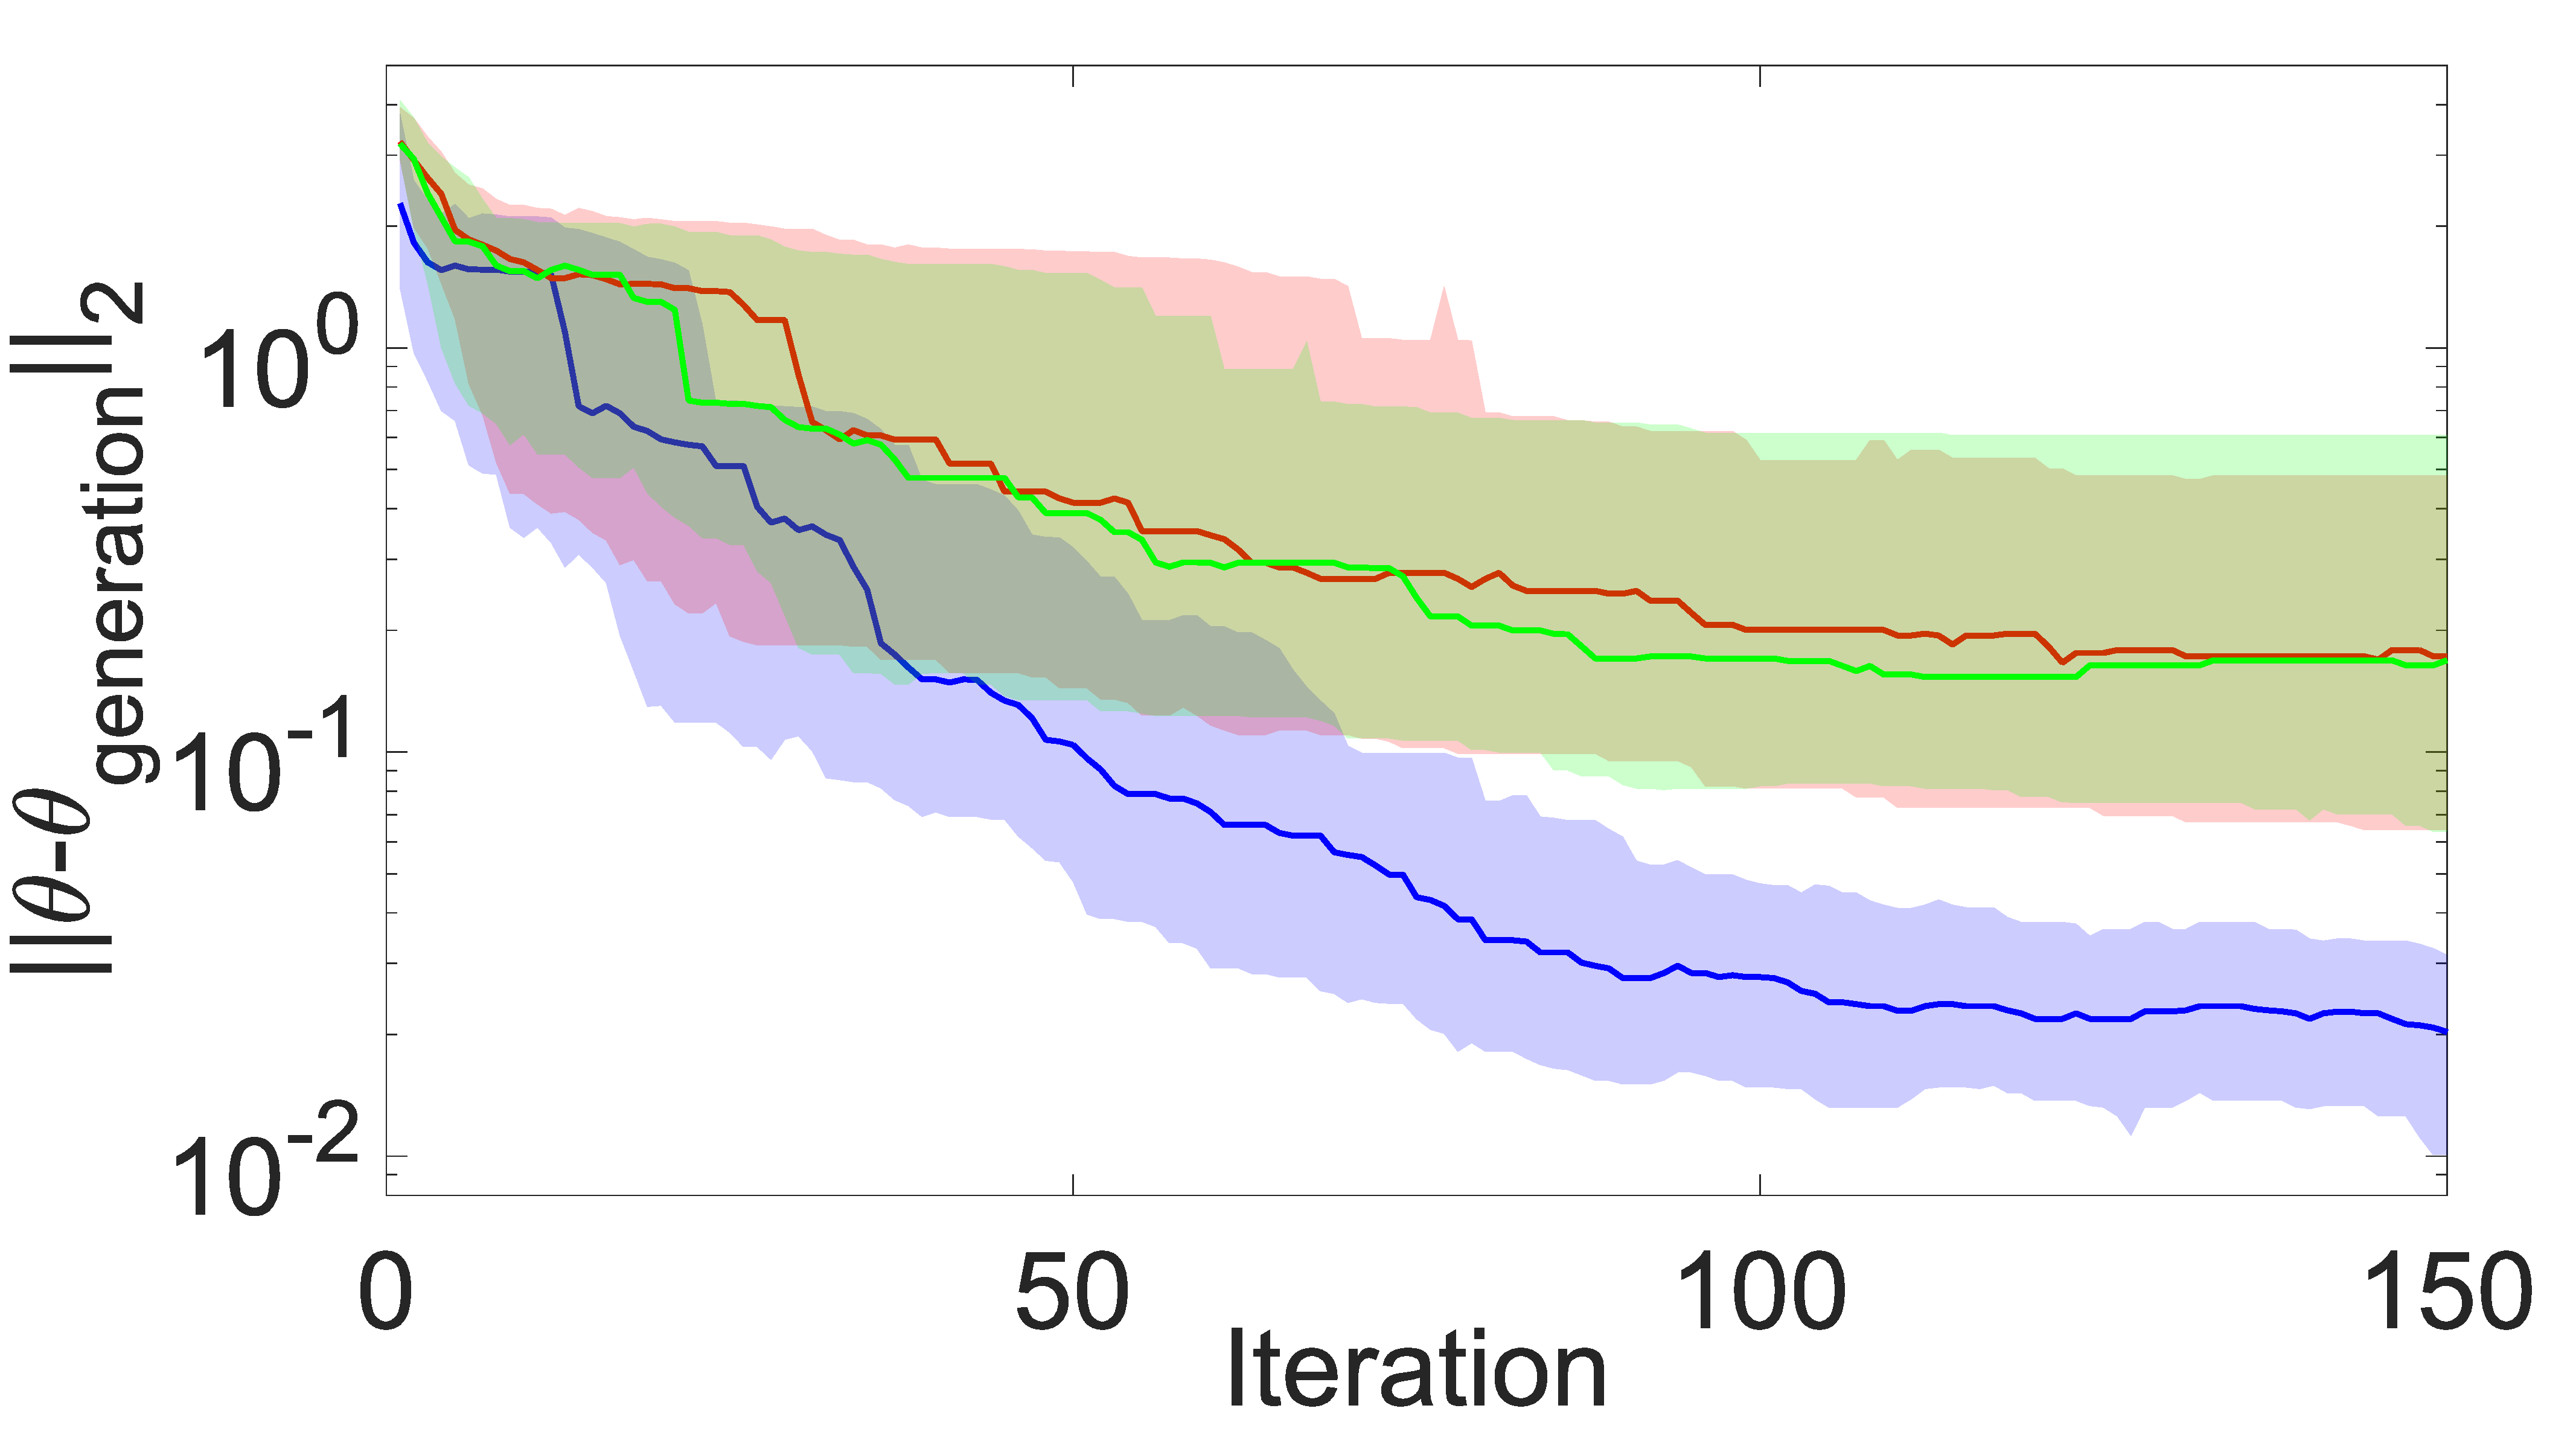
\includegraphics[width=2.72in]{chaos/chaos_distance.pdf}
	\caption{Convergence for transition dynamics parameters of the pickover attractor in terms of the cumulative best $\log p\left(Y,\theta\right)$ (\emph{left}) and distance to the ``true" $\theta$ used in generating the data (\emph{right}). Solid line shows median over 100 runs, whilst the shaded region the 25/75\% quantiles.  \label{fig:chaos}
		\vspace{6pt}}
\end{figure*}

\begin{figure}[p]
	\centering
	\begin{subfigure}[t]{0.48\textwidth}
		\centering
		
\includegraphics[height=5.6cm,width=6.4cm]{chaos/compressed/first_iter_alt.png}
		\caption{{$\begin{array}{c}
				\text{1 iteration}, \; 
				\theta = [-1.478,0.855]^T 
				\end{array}$}}
	\end{subfigure}
	\begin{subfigure}[t]{0.48\textwidth}
		\centering
		\tiny
		
\includegraphics[height=5.6cm,width=6.4cm]{chaos/compressed/20_iter_alt.png}
		\caption{{$\begin{array}{c}
				\text{20 iterations}, \; 
				\theta = [-2.942,1.550]^T 
				\end{array}$}}
	\end{subfigure}
	\\
	\vspace{20pt}
	\begin{subfigure}[t]{0.48\textwidth}
		\centering
		\tiny
		
\includegraphics[height=5.6cm,width=6.4cm]{chaos/compressed/100_iter_altj.png}
		\caption{{$\begin{array}{c}
				\text{100 iterations}, \;
				\theta = [-2.306,1.249]^T 
				\end{array}$}}
	\end{subfigure}
	\begin{subfigure}[t]{0.48\textwidth}
		\centering
		\tiny
		
\includegraphics[height=5.6cm,width=6.4cm]{chaos/compressed/target_light.png}
		\caption{{$\begin{array}{c}
				\text{Ground truth}, \;
				\theta = [-2.3,1.25]^T
				\end{array}$}}
	\end{subfigure}
	\caption{A series of trajectories for different parameters, demonstrating convergence to the true attractor.  The colormap is based on the speed and curvature of the trajectory, with rendering done using the program Chaoscope (available at {\href{http://www.chaoscope.org/}{http://www.chaoscope.org/}}). \label{fig:chaoscope}}
\end{figure}

We next consider the case of learning the dynamics parameters of a chaotic attractor.  Chaotic attractors present an interesting case for tracking problems as, although their underlying dynamics are strictly deterministic with bounded trajectories, neighbouring trajectories diverge exponentially\footnote{It is beyond the scope of this paper to properly introduce chaotic systems.  We refer the reader to \cite{devaney1989introduction} for an introduction.}.  Therefore regardless of the available precision, a trajectory cannot be indefinitely extrapolated to within a given accuracy and probabilistic methods such as the extended Kalman filter must be incorporated \citep{fujii2013extended,ruan2003chaotic}. From an empirical perspective, this forms a challenging optimization problem as the target transpires to be multi-modal, has variations at different length scales, and has local minima close to the global maximum.

Suppose we observe a noisy signal $y_t \in \real^{K}, \; t = 1,2,\dots,T$ in some $K$ dimensional observation space were each observation has a lower dimensional latent parameter $x_t \in \real^{D},  \; t = 1,2,\dots,T$ whose dynamics correspond to a chaotic attractor of known type, but with unknown parameters.  Our aim will be to find the MMAP values for the dynamics parameters $\theta$, marginalizing out the latent states.  The established parameters can then be used for forward simulation or tracking.  

To carry out the required MMAP estimation, we apply BOPP to the extended Kalman smoother
\begin{align}
\label{eq:Kalman}
x_1 \sim & \mathcal{N} \left(\mu_1, \sigma_1 I\right) \\
x_t = & A \left(x_{t-1}, \theta\right)+\delta_{t-1}, \; & \delta_{t-1} \sim \mathcal{N} \left(0, \sigma_q I\right) \\
y_t = & C x_{t}+\varepsilon_{t}, \; & \varepsilon_{t} \sim \mathcal{N} \left(0, \sigma_y I\right)
\end{align}
where $I$ is the identity matrix, $C$ is a known $K \times D$ matrix,  $\mu_1$ is the expected starting position, and $\sigma_1, \sigma_q$ and $\sigma_y$ are all scalars which are assumed to be known.  The transition function $A \left(\cdot,\cdot\right)$
\begin{subequations}
	\begin{align}
	\label{eq:pickover}
	x_{t,1} = & \sin \left(\beta x_{t-1,2}\right)-\cos\left(\frac{5x_{t-1,1}}{2}\right)x_{t-1,3}  \\
	x_{t,2} = & -\sin \left(\frac{3x_{t-1,1}}{2}\right)x_{t-1,3}-\cos\left(\eta x_{t-1,2}\right) \\
	x_{t,3} = & \sin \left(x_{t-1,1}\right)
	\end{align}
\end{subequations}
corresponds to a Pickover attractor \citep{pickover1995pattern} with unknown parameters $\theta = \left\{\beta,\eta\right\}$ which we wish to optimize.  Note that $\eta$ and $-\eta$ will give the same behaviour.

Synthetic data was generated for $500$ time steps using the parameters of  $\mu_1 = [-0.2149,-0.0177,0.7630]^T$, $\sigma_1 = 0$, $\sigma_q = 0.01$, $\sigma_y = 0.2$, a fixed matrix $C$ where $K=20$ and each column was randomly drawn from a symmetric Dirichlet distribution with parameter $0.1$, and ground truth transition parameters of $\beta = -2.3$ and $\eta = 1.25$ (note that the true global optimum for finite data need not be exactly equal to this).  

MMAP estimation was performed on this data using the same model and parameters, with the exceptions of $\theta$, $\mu_1$ and $\sigma_1$.  
The prior on $\theta$ was set to a uniform in over a bounded region such that
\begin{align}
\label{eq:priorKalman}
p\left(\beta,\eta\right) = \begin{cases}
1/18, & \mathrm{if} -3 \le \beta \le 3 \; \cap \; 0 \le \eta \le 3\\
0, & \mathrm{otherwise}
\end{cases}.
\end{align}
The changes $\mu_1 = [0,0,0]$ and $\sigma_1 = 1$ were further made to reflect the starting point of the latent state being unknown.   For this problem, BOPP aims to maximize
\begin{align}
p(\beta,\eta | y_{t=1:T}) = \int p(\beta,\eta,x_{t=1:T} | y_{t=1:T}) \mathrm{d}x_{t=1:T} .
\end{align}
Inference on the transformed marginal query was carried out using SMC with 500 particles.  Convergence results are given in Figure~\ref{fig:chaos} showing that BOPP comfortably outperforms the PMMH variants, while Figure~\ref{fig:chaoscope} shows the simulated attractors generated from the dynamics parameters output by various iterations of a particular run of BOPP.
